\subsection{Data}
I will be modelling the velocity of the aeroplane, by taking account the forces that act on the aeroplane during the 26 seconds. By taking account the different forces that act on the plane during landing, i will be able to model the velocity and hence then find the area under the velocity time graph using integration to find the length of the runway required for the aeroplane to land safely.
\\
The data given shows how the velocity of the landing aeroplane changes with respect to time.  This data was collected from the MEI coursework bank and will be used to model the landing of an aeroplane in order to determine the length of a runway required for a landing aeroplane.
\\
An important point to note about the data is that each point has been rounded to the nearest integer. The significance of this is that, it means that when testing how a model performs against the data, if model is correct to the nearest integer for all values this would mean that the model is a good approximation for reality. 

\subsection{Graph of Data}

\begin{figure}[h]
\centering
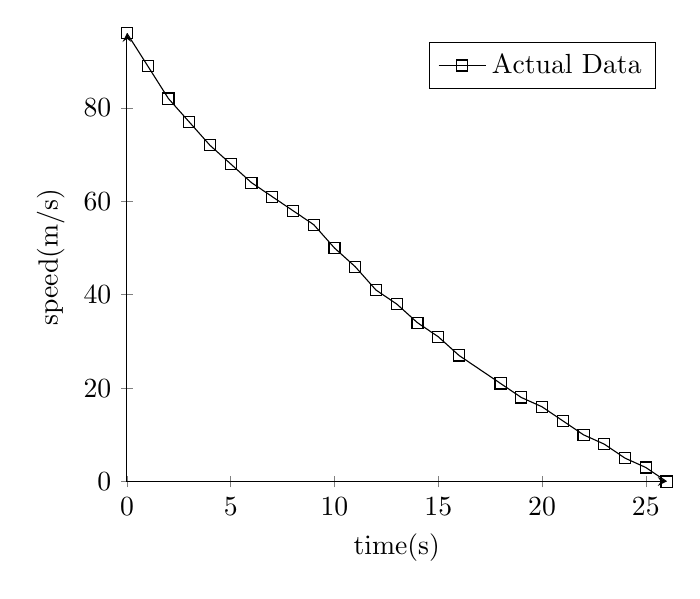
\begin{tikzpicture}
\begin{axis}[
    axis lines = left,
    xlabel = time(s),
    ylabel = speed(m/s),
]
 
 \addplot[
    color=black,
    mark=square]
    coordinates {(0,96)(1,89)(2,82)(3,77)(4,72)(5,68)(6,64)(7,61)(8,58)(9,55)(10,50)(11,46)(12,41)(13,38)(14,34)(15,31)(16,27)(18,21)(19,18)(20,16)(21,13)(22,10)(23,8)(24,5)(25,3)(26,0)};
\addlegendentry{Actual Data}

\end{axis}
\end{tikzpicture}
\caption{Table showing how the velocity of the plane changes with respect to time}
\end{figure}

\begin{flushleft}
\begin{table}[h]
\centering
    \begin{tabular}{|l|l|l|l|l|l|l|l|l|l|l|l|l|l|l|l|l|l|l|l|l|l|l|}
        \hline
        t(s) & 0 & 1 & 2 & 3 & 4 & 5 & 6 & 7 & 8 & 9 & 10 & 11 & 12 & 13 & 14 & 15\\ \cline{1-17} 
        Actual v(m/s) & 96 & 89 & 82 & 77 & 72 & 68 & 64 & 61 & 58 & 55 & 50 & 46 & 41 & 38 & 34 & 31 \\ \cline{1-17}
    \end{tabular}
    \caption{Velocity of the plane from $ 0 \leq t \leq 15$}
    \vspace{0.5cm}
    
    \begin{tabular}{|l|l|l|l|l|l|l|l|l|l|l|l|}
        \hline
        t(s) & 16 & 17 & 18 & 19 & 20 & 21 & 22 & 23 & 24 & 25 & 26 \\ \cline{1-12}
        Actual v(m/s) & 27 & 24 & 21  & 18 & 16 & 13 & 10 & 8 & 5 & 3 & 0 \\ \cline{1-12}
    \end{tabular}
    \caption{Velocity of the plane from $ 15 \leq t \leq 26$}
\end{table}
\end{flushleft}